\section{Ubalance i kapacitetsudnyttelse}
Ved kapacitetsmangel på OA er afdelingen nødsaget til at omstrukturere forholdet mellem aktivitet og kapacitet. Dette er mhp. at opnå en balance mellem de ressourcer og de krav, der stilles i den pågældende situation.\cite{Bjerg2016} %Generelt er personalet den begrænsende faktor for planlægning og kapacitetsudnyttelse\cite{Company2013}. 

\subsection{Arbejdsvilkår} \label{Per_sik}
%Hvordan påvirkes personalets arbejdsrutiner ved kapacitetsmangel? Hvor længes må deres arbejdsdag maksimalt være? Stiger antallet af fejl når personalet varetager en større arbejdsbyrde end planlagt? Hvor omkostningsfuldt er det? 

I tilfælde af kapacitetsmangel er der udarbejdet en arbejdstilrettelæggelse af Region Nordjylland for personalet på OA. Ved kapacitetsmangel påtager lederen, eller dennes stedfortræder, ansvaret for at finde en løsning på dette problem. Dette kan betyde, at det afgående vagthold skal blive indtil en midlertidig løsning er fundet eller en tidligere indkaldelse af det næste vagthold skal forekomme. I nogle tilfælde kan det være nødvendigt at låne ressourcer fra andre afsnit eller indkalde personale fra vikarbureauet. Derudover undersøges det, hvorvidt behandlingen af elektive patienter kan udskydes.\cite{Bjerg2016} 
Hvis der derimod er flere sengepladser end patienter, betyder dette, at der ikke er fuld udnyttelse af personalets arbejdskraft.

Pauser, i perioder med kapacitetsmangel, afholdes således de passer ind i arbejdsrytmen og nogle dage holdes der ikke pauser. Herudover kan sygeplejerskene tilkaldes fra en pause, hvis det er nødvendigt.[\ref{bilagA}] Ved overarbejde må en arbejdsuge for en sygeplejerske, ifølge arbejdstidsaftalen indgået med Dansk Sygeplejeråd, ikke overstige 48 timer. Hvis sundhedspersonalet er nødsaget til at arbejde længere end den normale arbejdstid, viser dette sig at have en negativ indvirkning på personalets arbejdesopgaver\cite{Dinges2004}. Overarbejde kan resultere i en presset arbejdsdag og dermed en forringet kvalitet af behandlingen. Hver anden regionalt ansat sygeplejerske på tværs af regionerne mener dertil, at den travle arbejdsdag påvirker patienternes sikkerhed.\cite{Kjeldsen2015}


\subsection{Patientsikkerhed}\label{patsik}
%Hvordan påvirker kapacitetsmangel ift. brandsikkerhed? Laver personalet flere fejl, som går ud over patienterne ved overbelægning? Hvordan fungerer omrokering af patienter (gangarealer, vaskerum ect.)? Hvor omkostningsfuldt er det for OA’s budget? brandsikkerhed og Genindlæggelse
Under perioder med kapacitetsmangel er det ofte nødvendigt at overflytte patienter til andre afsnit, gangarealer eller fyldte stuer. Det er typisk patienter, der snart udskrives, der overflyttes. Ved flytning af patienter, flyttes de indbyrdes mellem afdelingens afsnit eller til andre matrikler i eksempelvis Farsø, Hjørring eller Frederikshavn. Overordnet ønskes det at beholde børn, traume- og rygpatienter på afdelingen. Eksempelvis kan der ved rygpatienter opstå ændringer samt komplikationer ift. udstyr og varetagelse, hvilket kan resultere i, at patienten er nødsaget til at starte forfra med forløbet.[\ref{bilagO2}] Ved overflytning til andre matrikler er det oftest færdigtbehandlede patienter, der kan starte på genoptræning eller videre mobilisering.[\ref{bilagA}] Overflytningen kan belaste både fysiske og psykiske forhold for patienter såvel som pårørende\cite{Heidmann2014}. Herunder kan skærpet privatliv forekomme hos patienter, der er flyttet til gangarealer eller fyldte stuer\cite{Madsen2014}. 

Som nævnt forringes kvaliteten af behandlingen ved overarbejde, hvor det ligeledes ses, at mortalitetsraten øges med $1,2~\%$ ved en overskridelse af belægningen med $10~\%$\cite{Madsen2014}. Hertil understreges det, at der kan være ukendte parametre, der påvirker mortalitetsraten, og det nødvendigvis ikke er belægning, der er den primære årsag til en øget mortalitet. For at undgå forringet kvalitet af behandling forsøges det at få patienter udskrevet tidligere, således et ønske om balance mellem aktivitet og kapacitet opnås.


Ved kapacitetsmangel tilkaldes en brandvagt til afdelingen, hvis dette har fundet sted i over $4$ timer, for således at sikre patienterne ved evakuering under brand. En brandvagt kan højest overvåge to afdelinger på samme etage, hvorfor det kan være nødvendigt, at der indkaldes flere.\cite{Beredskab2016}


\subsection{Optimering af kapacitetsudnyttelse}
Kapacitetsudnyttelsen kan angiveligt optimeres ved at ændre på én af parametrene under hhv. aktivitet og kapacitet. Herunder anses faktorer, såsom antallet af patienter samt personale som de parametre, der hurtigst kan justeres på for at opnå balance i kapaciteten. 

\subsubsection{Aktivitet}
Ift. aktivitet i kapacitetsudnyttelse anses antallet af patienter værende nemmest at regulere på. Aktivitetsaspektet vil herved reguleres, da der ved færre patienter vil forekomme færre kontakter, herunder forundersøgelse, behandling samt kontrol. Ved akut opstående tilfælde kan det derved være nødvendigt at udsætte patienter med det formål at kunne behandle akutte patienter.[\ref{bilagO1}]


\subsubsection{Kapacitet}
I kapacitetaspektet anses personale som værende den variabel, der er nemmest at regulere på. En større patientbyrde kan medvirke til en øget arbejdsbyrde for det tilstedeværende personale. Det kan derved, i svære tilfælde, være nødvendigt at tilkalde mere personale for at varetage arbejdsopgaver. 
Udover en regulering af personalet justeres der på disponible sengepladser for at opretholde kapaciteten på afdelingen. Af \figref{fig:sengepladser} fremgår reguleringen af sengepladser på OA over 35 måneder fra år 2014 til 2016.\cite{Bjerg2016}

\begin{figure}[H] 
\begin{center}
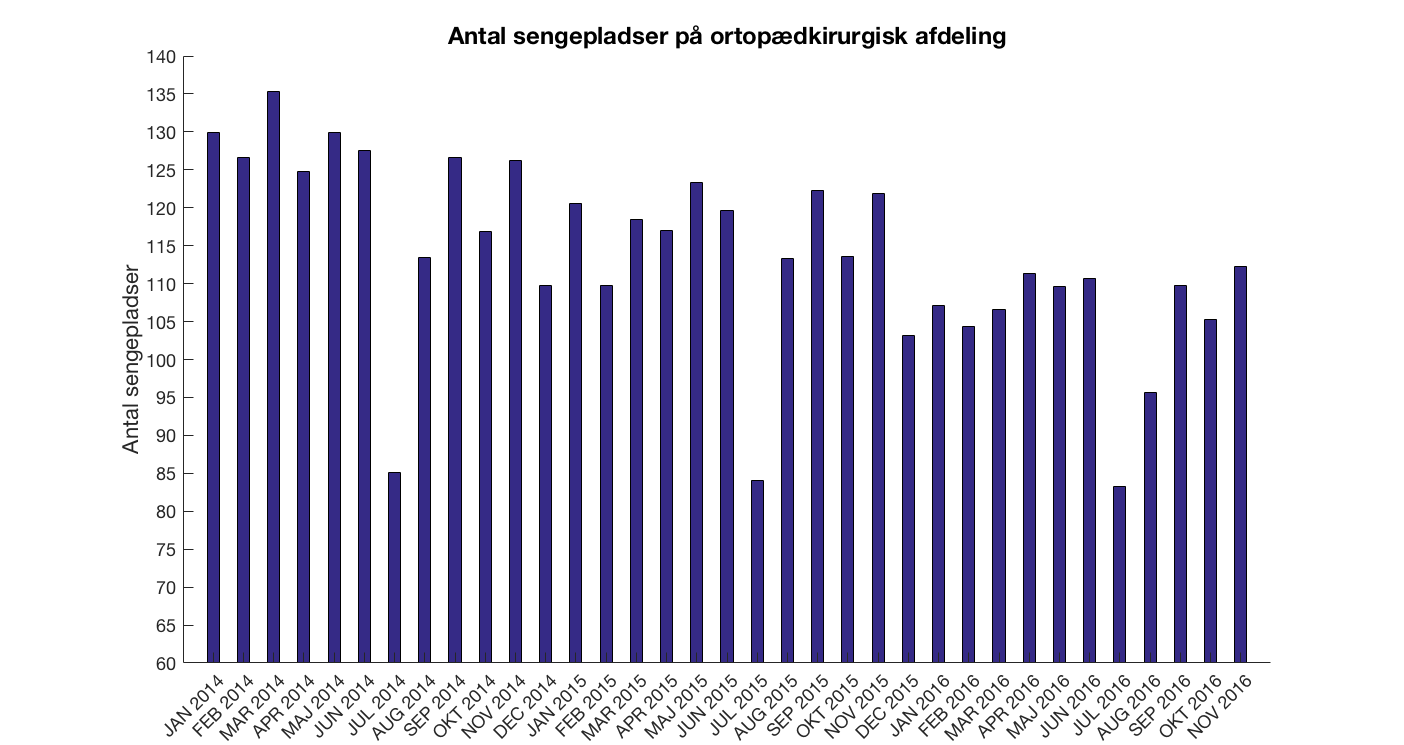
\includegraphics[width=0.8\textwidth]{figures/sengepladser}
\end{center}
\caption{textit{Disponible sengeplader pr. måned på OA over en periode fra januar måned år 2014 til november år 2016.}\cite{SDS2015}} 
\label{fig:sengepladser} 
\end{figure}

\noindent
Det fremgår af \figref{fig:sengepladser}, at de gennemsnitlige disponible sengepladser på OA varierer på månedsbasis. Sengepladserne er i gennemsnit faldet fra 121 til 105 fra år 2014 til 2016. Sengepladserne er derved faldet med 16 sengeplader over en 2 årig periode. I juli måned ses der færre disponible sengepladser, dette kan angiveligt skyldes, at personalet ønsker ferie denne måned. 

Opvågningsrum sætter ligeledes en begrænsning for afdelingens kapacitet, da der er begrænsede pladser til patienter efter en operation. Der kan således ikke startes nye operationer, hvis opvågningsrummet er fyldt, hvilket betyder, at personalet er nødsaget til at udskyde de planlagte operationer.[\ref{bilagO1}]

\section{Forudsigelse af indlæggelsesvarighed}
I år 2017 træder en ny budgetaftale i kraft på OA. Denne fokuserer bl.a. på balance mellem krav og ressourcer. Overordnet prioriteres hurtig udregning, bestående af sammenhængende patientforløb uden unødig ventetid og behandling af nordjyske borgere. Det ønskes ligeledes, at den gennemsnitlige ventetid til operation skal reduceres fra 57 til 50 dage.\cite{Budget2016}

På baggrund af foregående analyse samt den nye budgetaftale vurderes det, at OA har et voksende behov for et redskab til planlægning af elektive patienter. Et sådan redskab kan udarbejdes således, at indlæggelsesvarigheden forsøges forudsagt ud fra parametre. Dette vil give lægesekretæreren et overblik over de kommende ugers disponible sengepladser, hvilket giver et større vurderingsgrundlag for planlægning af elektive patienter.

\subsection{Parametre}
Indlæggelsesvarigheden for en patient påvirkes af flere parametre. Dette kan både være parametre, som kan påvirke indlæggelsesvarigheden før og efter en operation. Som tidligere nævnt afhænger kapacitetsudnyttelsen af forholdet mellem aktivitet og kapacitet. Under aktivitet kan patientens demografiske faktorer og livsstilsfaktorer have indflydelse på operationen og indlæggelsesvarigheden.
Patientens alder kan have betydning for komplikationer under en operation. Dette kan skyldes lavt funktionsniveau og muskeltab, som ofte er aldersbetinget. Yngre patienter med højt funktionsniveau har derimod ofte kortere indlæggelsesvarighed.\cite{Kehlet2001, Janssen2002}

Udover demografiske faktorer kan livsstilsfaktorer, såsom vægt, have en indflydelse på
operationer, da overvægt giver større risiko
for blodpropper\cite{Ermonds2004}. Ved overvægt anbefales det derved at tabe sig før
en eventuel operation. Foruden mindsket risiko ved opståede komplikationer, kan
smerter ligeledes reduceres ved vægttab.
Andre livsstilsfaktorer som eks. rygning kan have betydning
for komplikationer under operationer. Rygning kan være medvirkende til at knogler
og sår heler langsommere. Ved operationer, hvor der skal transplanteres knoglevæv, f.eks. rygoperationer, afhænger resultatet af operation af, at knoglevævet heler rigtigt.
Det anbefales derfor at stoppe med at ryge seks måneder før en operation. En anden livstilsfaktor, såsom et alkoholindtag over det anbefaldede, kan øge risikoen for blødning under operationer samt infektioner i såret.\cite{Nordjylland2014}
Yderligere kan kapacitet have indflydelse på patienters indlæggelsesvarighed. Dette kan være i form af mangel på personale pga. ferie, sygdom eller lignende. 
Derudover kan mangel på sengepladser ligeledes påvirke indlæggelsesvarigheden.
Foregående analyse leder således op til projektets problemformulering.



